%%%%%%%%%%%%%%%%%%%%%%%%%%%%%%%%%%%%%%%%%
% Masters/Doctoral Thesis
% LaTeX Template
% Version 2.3 (25/3/16)
%
% This template has been downloaded from:
% http://www.LaTeXTemplates.com
%
% Version 2.x major modifications by:
% Vel (vel@latextemplates.com)
%
% This template is based on a template by:
% Steve Gunn (http://users.ecs.soton.ac.uk/srg/softwaretools/document/templates/)
% Sunil Patel (http://www.sunilpatel.co.uk/thesis-template/)
%
% Template license:
% CC BY-NC-SA 3.0 (http://creativecommons.org/licenses/by-nc-sa/3.0/)
%
%%%%%%%%%%%%%%%%%%%%%%%%%%%%%%%%%%%%%%%%%

%----------------------------------------------------------------------------------------
%	PACKAGES AND OTHER DOCUMENT CONFIGURATIONS
%----------------------------------------------------------------------------------------

\documentclass[
11pt, % The default document font size, options: 10pt, 11pt, 12pt
%oneside, % Two side (alternating margins) for binding by default, uncomment to switch to one side
chapterinoneline,% Have the chapter title next to the number in one single line
english, % ngerman for German
singlespacing, % Single line spacing, alternatives: onehalfspacing or doublespacing
%draft, % Uncomment to enable draft mode (no pictures, no links, overfull hboxes indicated)
%nolistspacing, % If the document is onehalfspacing or doublespacing, uncomment this to set spacing in lists to single
%liststotoc, % Uncomment to add the list of figures/tables/etc to the table of contents
%toctotoc, % Uncomment to add the main table of contents to the table of contents
parskip, % Uncomment to add space between paragraphs
%nohyperref, % Uncomment to not load the hyperref package
headsepline, % Uncomment to get a line under the header
]{MastersDoctoralThesis} % The class file specifying the document structure

\usepackage[utf8]{inputenc} % Required for inputting international characters
\usepackage[T1]{fontenc} % Output font encoding for international characters

%\usepackage{palatino} % Use the Palatino font by default
\usepackage{fourier}

\usepackage{graphicx}
\usepackage{caption}
\usepackage{subcaption}
\usepackage{scrextend} % label-based lists
\addtokomafont{labelinglabel}{\sffamily}
\usepackage{siunitx}
\usepackage{mathtools}
\usepackage{amsmath}
\usepackage{mathtools}
\renewcommand{\vec}[1]{\mathbf{#1}} % in order to have the vectors in bold
\DeclarePairedDelimiter{\norm}{\lVert}{\rVert} % for the nice double bars

\usepackage[backend=bibtex,style=ieee,natbib=true]{biblatex} % Use the bibtex backend with the authoryear citation style (which resembles APA)

\addbibresource{example.bib} % The filename of the bibliography

\usepackage[autostyle=true]{csquotes} % Required to generate language-dependent quotes in the bibliography


%----------------------------------------------------------------------------------------
%	MARGIN SETTINGS
%----------------------------------------------------------------------------------------

\geometry{
	paper=a4paper, % Change to letterpaper for US letter
	inner=2.5cm, % Inner margin
	outer=2.5cm, % Outer margin
	bindingoffset=1.2cm, % Binding offset
	top=1.5cm, % Top margin
	bottom=1.5cm, % Bottom margin
	%showframe,% show how the type block is set on the page
}

%----------------------------------------------------------------------------------------
%	THESIS INFORMATION
%----------------------------------------------------------------------------------------

\thesistitle{Ensuring self-haptic Consistency for Immersive Amplified Embodiment} % Your thesis title, this is used in the title and abstract, print it elsewhere with \ttitle
\supervisor{Dr. Ronan \textsc{Boulic}} % Your supervisor's name, this is used in the title page, print it elsewhere with \supname
\examiner{} % Your examiner's name, this is not currently used anywhere in the template, print it elsewhere with \examname
\degree{MSc in Computer Science} % Your degree name, this is used in the title page and abstract, print it elsewhere with \degreename
\author{Sidney \textsc{Bovet}} % Your name, this is used in the title page and abstract, print it elsewhere with \authorname
\addresses{} % Your address, this is not currently used anywhere in the template, print it elsewhere with \addressname

\subject{} % Your subject area, this is not currently used anywhere in the template, print it elsewhere with \subjectname
\keywords{Vitual reality, Embodiment, Retargetting, Motion capture} % Keywords for your thesis, this is not currently used anywhere in the template, print it elsewhere with \keywordnames
\university{École Polytechnique Fédérale de Lausanne} % Your university's name and URL, this is used in the title page and abstract, print it elsewhere with \univname
\department{\href{http://ic.epfl.ch/en}{School of Coputer and Communication Sciences}} % Your department's name and URL, this is used in the title page and abstract, print it elsewhere with \deptname
\group{\href{http://iig.epfl.ch/}{Immersive Interaction Group}} % Your research group's name and URL, this is used in the title page, print it elsewhere with \groupname
\faculty{\href{http://ic.epfl.ch/computer-science}{Computer Science Section}} % Your faculty's name and URL, this is used in the title page and abstract, print it elsewhere with \facname

\hypersetup{pdftitle=\ttitle} % Set the PDF's title to your title
\hypersetup{pdfauthor=\authorname} % Set the PDF's author to your name
\hypersetup{pdfkeywords=\keywordnames} % Set the PDF's keywords to your keywords

\begin{document}

\frontmatter % Use roman page numbering style (i, ii, iii, iv...) for the pre-content pages

\pagestyle{plain} % Default to the plain heading style until the thesis style is called for the body content

%----------------------------------------------------------------------------------------
%	TITLE PAGE
%----------------------------------------------------------------------------------------

\begin{titlepage}
\begin{center}

{\scshape\LARGE \univname\par}\vspace{1.5cm} % University name
\textsc{\Large Master Thesis}\\[0.5cm] % Thesis type

\HRule \\[0.4cm] % Horizontal line
{\huge \bfseries \ttitle\par}\vspace{0.4cm} % Thesis title
\HRule \\[1.5cm] % Horizontal line

\begin{minipage}[t]{0.4\textwidth}
\begin{flushleft} \large
\emph{Author:}\\
{\authorname} % Author name - remove the \href bracket to remove the link
\end{flushleft}
\end{minipage}
\begin{minipage}[t]{0.4\textwidth}
\begin{flushright} \large
\emph{Supervisor:} \\
{\supname} % Supervisor name - remove the \href bracket to remove the link
\end{flushright}
\end{minipage}\\[3cm]

\large \textit{Submitted in fulfillment of the requirements\\ for the degree of \degreename}\\[0.3cm] % University requirement text
\textit{in the}\\[0.4cm]
\groupname\\\deptname\\[2cm] % Research group name and department name

{\large \today}\\[4cm] % Date
%\includegraphics{Logo} % University/department logo - uncomment to place it

\vfill
\end{center}
\end{titlepage}

%----------------------------------------------------------------------------------------
%	DECLARATION PAGE
%----------------------------------------------------------------------------------------

%\begin{declaration}
%\addchaptertocentry{\authorshipname}
%
%\noindent I, \authorname, declare that this thesis titled, \enquote{\ttitle} and the work presented in it are my own. I confirm that:
%
%\begin{itemize}
%\item This work was done wholly or mainly while in candidature for a research degree at this University.
%\item Where any part of this thesis has previously been submitted for a degree or any other qualification at this University or any other institution, this has been clearly stated.
%\item Where I have consulted the published work of others, this is always clearly attributed.
%\item Where I have quoted from the work of others, the source is always given. With the exception of such quotations, this thesis is entirely my own work.
%\item I have acknowledged all main sources of help.
%\item Where the thesis is based on work done by myself jointly with others, I have made clear exactly what was done by others and what I have contributed myself.\\
%\end{itemize}
%
%\noindent Signed:\\
%\rule[0.5em]{25em}{0.5pt} % This prints a line for the signature
%
%\noindent Date:\\
%\rule[0.5em]{25em}{0.5pt} % This prints a line to write the date
%\end{declaration}
%
%\cleardoublepage

%----------------------------------------------------------------------------------------
%	QUOTATION PAGE
%----------------------------------------------------------------------------------------

\vspace*{0.2\textheight}

\noindent\enquote{\itshape Thanks to my solid academic training, today I can write hundreds of words on virtually any topic without possessing a shred of information, which is how I got a good job in journalism.}\bigbreak

\hfill Dave Barry

%----------------------------------------------------------------------------------------
%	ABSTRACT PAGE
%----------------------------------------------------------------------------------------

\begin{abstract}
\addchaptertocentry{\abstractname} % Add the abstract to the table of contents

The Thesis Abstract is written here (and usually kept to just this page). The page is kept centered vertically so can expand into the blank space above the title too\ldots

This project explores the possibility of distorting movements in the context of a stroke reabilitation task presented as a target-reaching VR serious game.

\end{abstract}

%----------------------------------------------------------------------------------------
%	ACKNOWLEDGEMENTS
%----------------------------------------------------------------------------------------

\begin{acknowledgements}
\addchaptertocentry{\acknowledgementname} % Add the acknowledgements to the table of contents

The acknowledgments and the people to thank go here\ldots

\end{acknowledgements}

%----------------------------------------------------------------------------------------
%	LIST OF CONTENTS/FIGURES/TABLES PAGES
%----------------------------------------------------------------------------------------

\tableofcontents % Prints the main table of contents

%\listoffigures % Prints the list of figures

%\listoftables % Prints the list of tables

%----------------------------------------------------------------------------------------
%	ABBREVIATIONS
%----------------------------------------------------------------------------------------

%\begin{abbreviations}{ll} % Include a list of abbreviations (a table of two columns)
%
%\textbf{LAH} & \textbf{L}ist \textbf{A}bbreviations \textbf{H}ere\\
%\textbf{WSF} & \textbf{W}hat (it) \textbf{S}tands \textbf{F}or\\
%
%\end{abbreviations}

%----------------------------------------------------------------------------------------
%	PHYSICAL CONSTANTS/OTHER DEFINITIONS
%----------------------------------------------------------------------------------------

%\begin{constants}{lr@{${}={}$}l} % The list of physical constants is a three column table
%
%% The \SI{}{} command is provided by the siunitx package, see its documentation for instructions on how to use it
%
%	Speed of Light & $c_{0}$ & \SI{2.99792458e8}{\meter\per\second} (exact)\\
%%Constant Name & $Symbol$ & $Constant Value$ with units\\
%
%\end{constants}

%----------------------------------------------------------------------------------------
%	SYMBOLS
%----------------------------------------------------------------------------------------

%\begin{symbols}{lll} % Include a list of Symbols (a three column table)
%
%$a$ & distance & \si{\meter} \\
%$P$ & power & \si{\watt} (\si{\joule\per\second}) \\
%%Symbol & Name & Unit \\
%
%\addlinespace % Gap to separate the Roman symbols from the Greek
%
%$\omega$ & angular frequency & \si{\radian} \\
%
%\end{symbols}

%----------------------------------------------------------------------------------------
%	DEDICATION
%----------------------------------------------------------------------------------------

%\dedicatory{For/Dedicated to/To my\ldots}

%----------------------------------------------------------------------------------------
%	THESIS CONTENT - CHAPTERS
%----------------------------------------------------------------------------------------

\mainmatter % Begin numeric (1,2,3...) page numbering

\pagestyle{thesis} % Return the page headers back to the "thesis" style

% Include the chapters of the thesis as separate files from the Chapters folder
% Uncomment the lines as you write the chapters

% Chapter 1

\chapter{Introduction} % Main chapter title

\label{Chapter1} % For referencing the chapter elsewhere, use \ref{Chapter1}

%----------------------------------------------------------------------------------------
%	SECTION 1
%----------------------------------------------------------------------------------------

In order to properly introduce this project we need to briefly cover multiple subjects, ranging from stroke rehabilitation to motion capture techniques. All these seemingly different subjects revolve around the idea that we can do something to help stroke patients recover faster by having them participate to serious Virtual Reality (VR) games in which their movements are distorted to keep them motivated.

\section{Stroke Rehabilitation}
%Explanation of what a stroke is and how to recover.
As explained by the NHLBI\footnote{National Heart, Lung, and Blood Institute: \url{https://www.nhlbi.nih.gov/health/health-topics/topics/stroke} [Last visited: 08.01.2017]}, a stroke is a medical condition occurring when parts of the brain stop being provided with proper blood flow. Without such oxygenation, brain cells quickly die. The resulting brain damage may induce various symptoms, such as loss of vision to one side or paralysis. It is the latter that is of interest to us, and more precisely the motor recovery process involved after the stroke itself has been identified and treated. As exposed by \cite{vos2015global}, there were more than 10 million stroke cases in 2013, which represents an increase of around 60-75\% with respect to 1990.

The motor recovery process involves so-called constraint-induced movement therapy, a technique that is at least around 100 years old as proposed by Oden \cite{oden1918systematic} in 1918. In his experiment he remarked that monkeys that were forced to use their almost-paralyzed limb through binding of the other one recovered much faster than the ones with unbound arms. This rather archaic procedure has been improved over the years, but it still exploits the same idea: it takes advantage of neuroplasticity and involves movement exercises of the paralyzed limb. The more the movements are exercised the better the motor recovery will be.

The process as a whole is a long one, involving checkups and exercises at both the hospital and home. Many factors play a role in how successful the recovery process will be, one of them and maybe the most important one being motivation. As argued by \cite{flores2008improving}, the more a patient participates to a rehabilitation task the greater the motor recovery will be. Keeping participants motivated during such tasks is thus essential.

\section{Virtual Reality}

We now jump to a completely different topic, but a careful reader will quickly understand how both are closely linked and of interest to us.

Virtual Reality can be defined as ``The computer-generated simulation of a three-dimensional image or environment that can be interacted with in a seemingly real or physical way by a person using special electronic equipment, such as a helmet with a screen inside or gloves fitted with sensors.'' \cite{oxford2015} The most common type of VR device used nowadays are Head-Mounted Displays (HMD), wich are constructed as a screen in front of which two lenses are fixated, allowing the device to be held in front of the eyes while focusing the screen's content at infinity. Coupled with inertial sensors, such device allows one to look around at a virtual environment. Other VR displays also exist, such as the CAVE: a cube with screen-faces surrounding a user proposed by \cite{cruz1992cave}. In the recent days, companies such as Oculus VR and HTC have begun commercializing HMD and VR becomes more widespread than ever.

\subsection{Immersion, Embodiment, and Presence}
As VR becomes more and more accessible to the general public and broadly used in the industry, the accepted meaning of the following terms sometimes diverged from their original definitions. As an effort to clarify these, here is a summary of the concepts these words describe.

\subsubsection{Immersion}
This first word unfortunately is the least understood by the general public. Immersion has a clear definition offered among others by \cite{slater2003note,sanchez2005presence} that we think is preferable to be recalled here: it refers to the capability of a system to deliver a convincing set of sensory stimuli. It is an objective measurement of parameters such as screen resolution, audio equipment, and sensors used.

\subsubsection{Embodiment}
\label{sec:embodiment}
Embodiment is defined in the field of cognitive neuroscience and philosophy of the mind by \cite{blanke2009full,debarba2017embodiment}. It encompasses the relevance of sensorimotor skills and the role the body has in shaping the mind, as well as the subjective experience of using and `having' a body. It is formally defined by \cite{de2011embodiment} as follows: ``E is embodied if some properties of E are processed in the same way as the properties of one’s body''.

One may from that perspective embody a tool, such as a pen or a hammer, even though that tool is not considered as being part of one's body. As described by \cite{de2011embodiment}, the \textit{sense} of embodiment (SoE) refers to the fact that one \textit{feels} such phenomena as opposed to only \textit{knowing} that it exists. As an example, learning that an organ is part of our body makes us embody that organ even though we cannot feel it, whereas felling like the tip of our pen actually is part of our hand creates a SoE towards that pen.

One key factor of the SoE is the \textbf{Sense of Agency}. It is defined by Tsakiris et al.\ \cite{tsakiris2006having} as ``the sense of intending and executing actions, including the feeling of controlling one’s own body movements, and, through them, events in the external environment.'' To continue with our pen example, the fact that one feels like controlling the position and pressure of the pen on a sheet of paper contributes to the SoE towards that pen. The Sense of Agency is therefore closely linked to our research topic, given that we aim at changing the way one interacts with a virtual environment by distorting the movements of the controlled virtual body. We are therefore acting directly on the foundations of the Sense of Agency.

Although of lesser interest to us, it should be noted here that the SoE rises from two other components, alongside Agency: the \textbf{Sense of Body ownership} and the \textbf{Sense of Self-Location}. The two following definitions are the ones proposed by Kilteni et al.\ \cite{kilteni2012sense}. Body ownership denotes the attribution of a body as our own. The sense arising from it comes twofold: receiving sensory information from that body, and the cognitive action of processing such information. The Sense of Self-Location on the other hand describes the feeling that our body occupies a given volume in space, that we \textit{are inside} a body. We are used to all of these senses because they are a given in the real world---unless one is injured or hindered in some way or another---but they may be manipulated using VR, in the same way we affect the Sense of Agency in our work.

\subsubsection{Presence}
What most people tend to call immersion actually is the sense of presence, described by \cite{held1992telepresence,slater1993representations} as the "sense of being there". As explained by \cite{debarba2017embodiment}, the central concept of the state of presence is that despite \textit{knowing} that it is a simulation, the user \textit{acts in} and \textit{reacts to} the virtual environment as if it were real.

\subsection{Haptics and Self-haptics}

`Haptic' relates to the sense of touch, and more specifically to the one associated to manipulating objects. Feeling the pressure of a sphere between one's fingers when grasping a ball is a haptic feedback. Self-haptic similarly denotes the haptic feedback of touching one's own body part. The feedback thus is dual: by touching one's own arm the brain will receive both the information of the hand touching something and the arm being touched by something. Moreover, before the contact even occurs the brain predicts such self-contact using proprioceptive information about the position of both body parts in space, and is thus very sensitive to such feedback inconsistency.

\section{Motion Capture}
\label{sec:mocap}
Motion capture can be defined as the action of capturing one's movements in order to reproduce such a motion in one context or another. Video game animations for instance are often performed by actors, whose walking or fighting movements are captured and then played back on the game's characters. The captured movement is often slightly altered, e.g.\ in order to fit it onto an avatar of different morphology, as proposed by \cite{molla2017egocentric}.

\section{Amplified Embodiment}

The concept of amplified embodiment can easily be understood as the merging of both Sections \ref{sec:embodiment} and \ref{sec:mocap}. By capturing one's movements and transposing those on an avatar, we may create a SoE towards that avatar. The goal of amplified embodiment is to distort that avatar's movements by amplifying them while preserving the SoE, which might be partially or completely lost if the distortion is too heavy or non-continuous for instance.

\section{Serious Games}

To conclude this chapter we take a quick look at another distinct topic, one that closes the loop and creates a connection between stroke rehabilitation, VR, motion capture, and amplified embodiment.

As defined by \cite{djaouti2011classifying,chen2005proof}, a serious game is a game that neither has entertainment, enjoyment, nor fun as its primary purpose. Instances of serious games include educational ones such as Blupi at Home\footnote{\url{http://www.ceebot.com/blupi/maison-e.php} [Last visited: 08.01.2017]}, a 1988 video game where young children could learn the alphabet by exploring a house with a yellow, egg-shaped character and playing various mini games. A more recent example is the ``Zombies, Run!''\footnote{\url{https://zombiesrungame.com/} [Last visited: 08.01.2017]} application, which is a running mobile application using storytelling coupled with GPS localization to keep people motivated at running outside.

We hope that by now the thread linking all of the above subjects is clear enough: we are interested in discovering by how much we can distort one's movements in the context of a VR serious game aimed at motor recovery while altering the sense of embodiment as little as possible, with the goal of keeping the patients motivated at performing the rehabilitation task.

% Chapter Template

\chapter{Related Work} % Main chapter title

\label{Chapter2} % Change X to a consecutive number; for referencing this chapter elsewhere, use \ref{ChapterX}

\section{Motion Capture and Inverse Kinematics}

Reference to \cite{molla2013singularity} and \cite{molla2017egocentric}.

\subsection{Egocentric Coordinates}

More details on \cite{molla2017egocentric} and \cite{molla2016precise}.

\section{Stroke Rehabilitation}

Stroke rehabilitation techniques and research. Talk about \cite{flores2008improving} and others.

% Chapter Template

\chapter{Implementation} % Main chapter title

\label{Chapter3} % Change X to a consecutive number; for referencing this chapter elsewhere, use \ref{ChapterX}

In this chapter we describe how we adapted the preexisting motion capture software in order to obtain the desired distorted behavior.

\section{Distortion model}

\subsection*{Linear Function}

As briefly mentioned in chapter \ref{Chapter2}, we are taking advantage of the Egocentric Coordinate formalism in order to introduce our distortion model. We modify each relative displacement vectors $\vec{v}_i$ according to some value $\gamma$. A distorted position $\vec{p}_j$ is thus obtained using equation \ref{eq:DistortionOperation}, which has been obtained by modifying the definition proposed by \cite{molla2017egocentric}, using a function that we are going to detail in the next few lines.

\begin{equation}
\label{eq:DistortionOperation}
\vec{p}_j = \displaystyle\sum_{i=1}^{n} \hat{\lambda}\big(\vec{x}_i + f(\vec{v}_i,\gamma )\big)
\end{equation}

\noindent
For ease of experimentation and understandability, we are looking for a linear function $f(x) = ax + b$. Figure \ref{fig:armExamples} gives an example of what we aim to achieve, while Figure \ref{fig:plotsOfGamma} below gives a more mathematical point of view of the distortion we are looking for, especially in terms of $a$, the slope of the function. This plot, as well as all of the other plots of this report, were obtained using the Plotly API \cite{plotly}.

\begin{figure}[h]
    \center{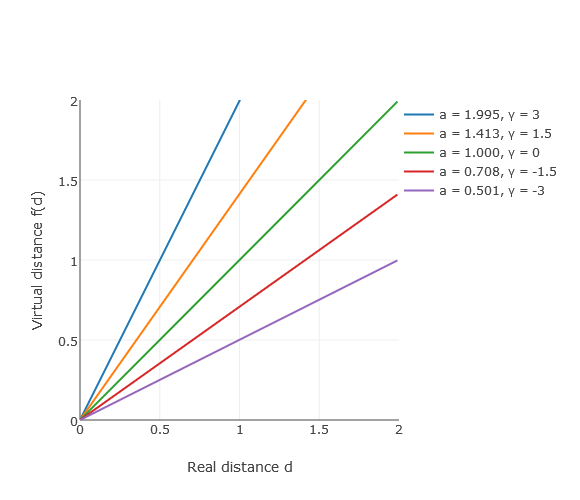
\includegraphics[width=.7\textwidth]
    {Figures/gamma_values.png}}
    \caption{An example of a few distortion functions for various values of slope $a$ and gain $\gamma $.}\label{fig:plotsOfGamma}
\end{figure}

\noindent
First of all we want to preserve self-haptic contacts. Such contact happens when a relative displacement vector $\vec{v} = \vec{0}$, which means that we need $f(0) = 0$, and thus $b = 0$.
\\\\
Intuitively, the slopes should be arranged around 1 which we want to correspond to $\gamma = 0$. One can also figure out that there is a correspondence between slopes below and above the line $f(x) = x$. For instance, for a given virtual distance to cover, a slope of \num{0.5} makes the traveling distance twice as long, whereas a slope of \num{2} halves the required movement.
\\\\
Formally, we are modifying each relative displacement vector as specified in Equation \ref{eq:DistortionOperation}, with $\gamma$ representing a gain, measured in \SI{}{\decibel}, and $f$ defined as:

\begin{equation}
\label{eq:DistortionFunction}
f(\vec{v},\gamma ) = \hat{v} \cdot \norm{\vec{v}} \cdot 10^{\frac{\gamma}{10}}
\end{equation}

\noindent
Where $\vec{v}$ is a vector, $\hat{v}$ is its normalized counterpart, and $\gamma \in \mathbb{R}$. The last factor, $10^{\frac{\gamma}{10}}$, comes from the definition of a gain, in \SI{}{\decibel} \cite{book:decibel}, based on two values $P_1$ and $P_2$ of a single, yet undefined unit:

\begin{align*}
    \text{gain} = \gamma &= 10 \cdot \log_{10} (\frac{P_1}{P_2})\\
    \frac{\gamma}{10} &= \log_{10} (\text{slope})\\
    \text{slope} &= 10^{\frac{\gamma}{10}}.
\end{align*}

\noindent
A value of $\gamma = 3$ thus indicates that the virtual movement will roughly be twice the amplitude of the registered one ($1.995 \approx 2$), while a gain of $\gamma = -3$ means one will have to travel twice as big (\num{0.501}) as a perceived distance in order to cover it. Figure \ref{fig:armExamples} shows two examples of distortion, and Figure \ref{fig:plotsOfGamma} gives a few instances of distortion functions with varying $\gamma $ values.

\begin{figure}
    \centering
    \begin{subfigure}[b]{0.2\textwidth}
        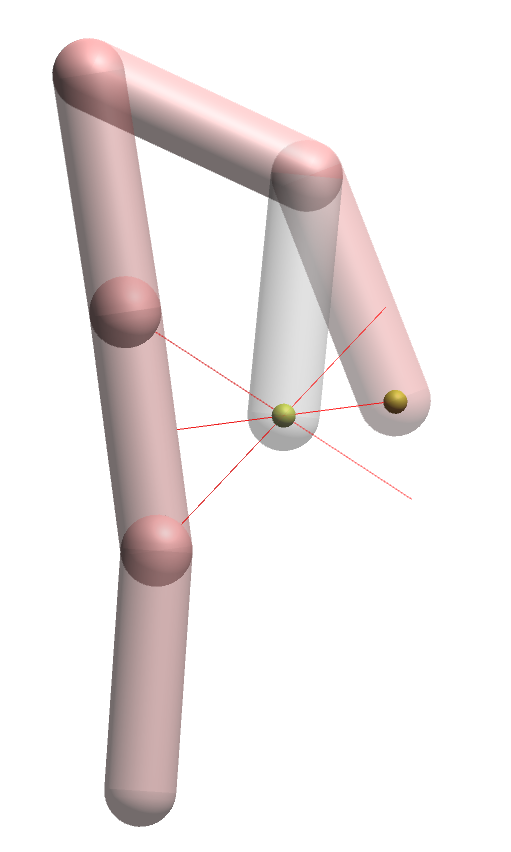
\includegraphics[width=\textwidth]{Figures/simple_distortion_3.png}
        \caption{$\gamma = 3$}
    \end{subfigure}
    ~ %add desired spacing between images, e. g. ~, \quad, \qquad, \hfill etc.
    %(or a blank line to force the subfigure onto a new line)
    \begin{subfigure}[b]{0.2\textwidth}
        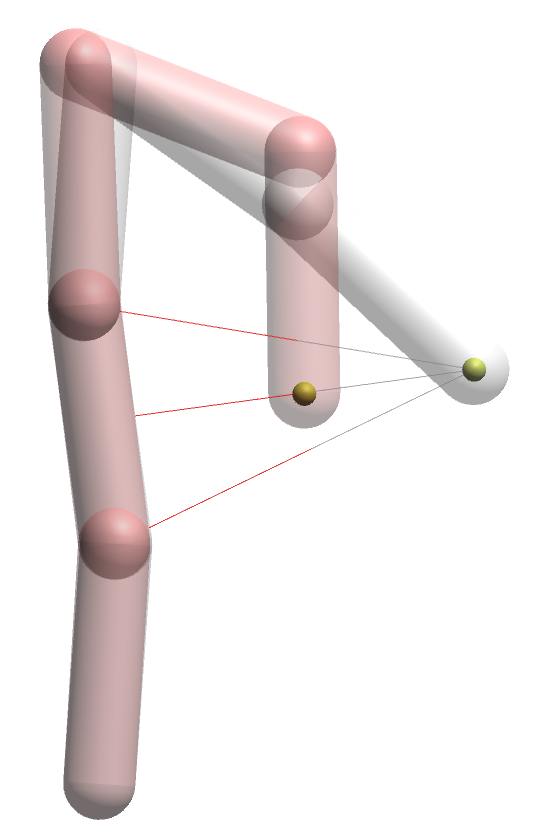
\includegraphics[width=\textwidth]{Figures/simple_distortion_-3.png}
        \caption{$\gamma = -3$}
    \end{subfigure}
    \caption{Two examples of distortion applied to a simple IK arm with multiple segments. The gray lines are the relative displacement vectors and the red ones are their distorted counterparts. Similarly, the gray arm represents the pose the real arm would take whereas the red one shows the resulting distorted pose. }\label{fig:armExamples}
\end{figure}

\subsection*{Other Functions}

Before deciding to use a simple, thus easier to quantify, linear function for our experimentation process, we tried out different functions that we think are of interest for further applications. Two of these functions are described here as a reference for further investigation.
\\\\
Description and plots of the Power and Cosine functions.

\section{Egocentric Coordinates}

We added one more modification to the definition of the position proposed by \cite{molla2017egocentric} which we modified to obtain Equation \ref{eq:DistortionOperation}, and more precisely the way $\lambda $ is defined. As explained in Appendix A.4 of \cite{molla2016precise}, it is originally computed as the product of two importance factors, proximity and orthogonality respectively denoted $\lambda_p$ and $\lambda_\bot $.
\\\\
Given that the justification for the latter factor mainly relies on the semantic information it conveys, and considering that it would introduce complex behaviors in the distortion, we decided to remove it. As an example, having the hand at a given distance of the chest and changing only its orientation with respect to that body part would cause that hand's position to be affected differently by other nearby body parts and thus be altered by our distortion model.
\\\\
The former importance factor was initially defined as $\lambda_p = \frac{1}{\norm{\vec{v}}}$. In practice we find that this formula does not give enough importance to nearby body parts, and we decided to change it slightly as $\lambda_p = \frac{1}{\norm{\vec{v}}^2}$. --Mention angle solide.-- % which more closely represents the amount of surface of an object that is visible at a distance $\norm{\vec{v}}$.

\section{Reachable Sphere}

A few words on the concept of reachable sphere and how it might help at the limits of the reachable space.

% Chapter Template

\chapter{Experiment} % Main chapter title

\label{Chapter4} % Change X to a consecutive number; for referencing this chapter elsewhere, use \ref{ChapterX}

We are trying to estimate the limits of self attribution of a distorted movement. We will do so by estimating the just noticeable difference (JND) in visual stimuli discrepancy. This means estimating the just noticeable \textit{distortion} made to the movement and hence the visual stimuli. The JND is estimated by using the adaptive staircase method introduced by Meese \cite{meese1995using}.

This method tries to estimate the JND by finding the point at which the subjects are uncertain whether a given visual stimuli corresponds to the actual movement they performed. These are found by changing the intensity of the distortion, based on whether the subject judged the last trial as distorted or not, and the JND is computed as the mean of the last few staircase turns (i.e.\ going from an increasing trend to a decreasing one or vice-versa). The detection judgment is gathered using a Yes/No prompt called the detection question : "Did the movements you saw exactly correspond to the movements you performed?"

\section{Just Noticeable Difference}

The JND will be measured in term of $\gamma$, the gain of the distortion function introduced in Equation \ref{eq:DistortionFunction}. In general, if $\gamma = \SI{-3}{\decibel}$ the subjects are hindered by having to travel two times the distance between the targets, whereas if $\gamma = \SI{3}{\decibel}$ the movement will be amplified and the required motion will be reduced by $50\%$.

Due to the nature of the Egocentric Coordinates and how the distortion is applied (respectively detailed in Chapters \ref{Chapter2} and \ref{Chapter3}), this will not exactly be a metric of the difference in the distance that the subjects have to cover in order to reach the target, such as the metric used by \cite{debarba2017embodiment}. It however gives a good understanding of the strength and the effect of the applied distortion.

\section{Equipment and Software}

The HMD used for this experiment is the Oculus Rift in its first consumer version, with a resolution of $1080 \times 1200$ pixels per eye and a refresh rate of \SI{90}{\hertz}.

---Some more words on head and body tracking, with references to \cite{molla2013singularity}.---

\section{Experiment design}

We manipulate three factors: the sign of the distortion (positive or negative), respectively yielding a helped and hindered movement, the starting value of that distortion (either \num{0} or \SI{9}{\decibel}, and the target sequence (see below). Chapter \ref{Chapter3} gives a complete overview of the concept of distortion and its sign, as well as how it is implemented.

\subsection{Task}
\label{sec:task}
While the whole set of IK goals will be distorted during the experiment, we will be focusing on the dominant hand movement. The task is performed in a seated position in order to avoid any unnecessary movement of the lower limbs, and has the subjects reach three targets. One of them may be in the air in front of them, while the starting and finishing location is the same relative to their skin. The reaching task is performed with the directing hand, and the subjects are instructed to keep their other hand at their side.

\begin{wrapfigure}{r}{.35\textwidth}
    \center{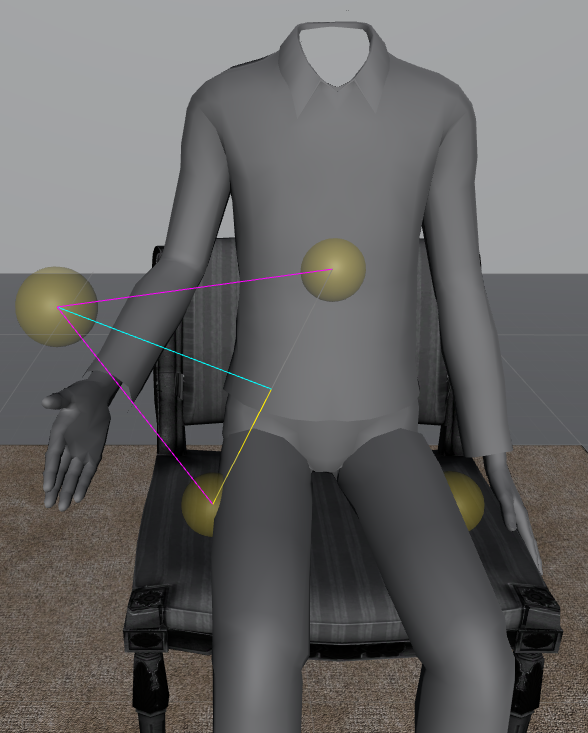
\includegraphics[width=.34\textwidth]
    {Figures/target_placement.png}}
    \caption{An example of target placement with lines showing how its position was reconstructed. The magenta lines are the one of desired length.}\label{fig:targetPlacement}
\end{wrapfigure}

There are four different target orders: \textbf{Chest-Air-Chest} ($O_1$), \textbf{Leg-Air-Leg} ($O_2$), \textbf{Chest-Leg-Chest} ($O_3$), and \textbf{Leg-Chest-Leg} ($O_4$). Both chest and leg targets are located as depicted on Figure \ref{fig:targetPlacement} and are picked according to the subject's handedness: left-handed subjects for instance will have to reach for their left thigh and right shoulder. The first target to be displayed, $T_1$, is always one on the skin and requires the subjects to perform a self-contact in order to activate it. After a random time between \num{200} and \SI{300}{\milli\second}, the target activates. Then the subject moves the hand to the next target, which activates after \SI{100}{\milli\second}. Once this is done the subject goes back to $T_1$, and the detection question is finally asked.

If the sequence requires an intermediary air target, its position is computed such that the subjects have to move a predefined distance $d = 75\%$ of arm length between $T_1$ and $T_{\text{air}}$. Given that a whole sphere of positions is possible, and in order to disambiguate that position, we require that $T_\text{air}$ is also at the same distance $d$ from the third, unused target $T_3$. The air target position therefore is on the intersection between the two spheres of radius $d$ centered on $T_1$ and $T_3$, and we chose the topmost position as a reasonable last disambiguation criterion. Figure \ref{fig:targetPlacement} shows how such position is computed.

One trial---or staircase run---consists of a reaching task, followed by the detection question. Based on the answer to this question, the experiment software modifies the distortion for the next staircase run as follows:
\begin{quote}
    \begin{labeling}{"No" and $\gamma = 0$}
      \item ["Yes"] The discrepancy is increased.
      \item ["No" and $\gamma \neq 0$] The discrepancy is decreased.
      \item ["No" and $\gamma = 0$] The parameter is not changed\footnote{We do not change the distortion in this case because this would invert the sign of the distortion, thus introducing a different distortion.}.
    \end{labeling}
\end{quote}

The amount of each increment or decrement is dynamic: it starts at \num{0.5} and is halved after the first staircase turn. That value is then kept for the rest of that staircase. The staircase is completed either when the subjects change direction 7 times or when they performed 20 trials in that staircase. Figure \ref{fig:trials} shows four instances of ten consecutive trial, depicting the four different initial staircases configuration used for each possible target order.

\begin{figure}[h]
    \center{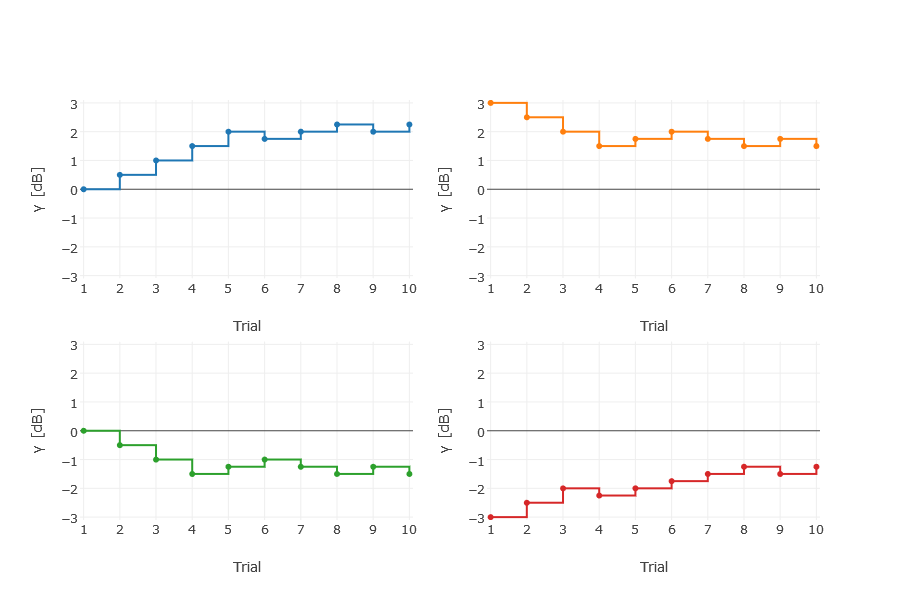
\includegraphics[width=\textwidth]
    {Figures/trials.png}}
    \caption{Four made up partial instances of staircases. Each one features ten trials and four staircases turns, including the one happening in the last trial. The sign of the staircase is the same for each row, while the starting distortion is the same for each column.}\label{fig:trials}
\end{figure}

\section{Hypotheses}

Considering the target orders $O_n$  we introduced in Section \ref{sec:task} and their resulting JNDs, denoted $\text{JND}_n$, the hypotheses we have for the experiment are the following:

\begin{quote}
    \begin{labeling}[:]{H2}
      \item [H1] The absolute value of the JND will be higher when the distortion is positive.
      \item [H2] For a positive distortion, $\text{JND}_3 \approx \text{JND}_4$
      \item [H3] Also for a positive distortion, $\text{JND}_1 < \text{JND}_2 < \text{JND}_3$
      \item [H4] For a negative distortion, $\text{JND}_1 > \text{JND}_2$
    \end{labeling}
\end{quote}

H1 is based on the findings of \cite{debarba2017embodiment}, who found that a hindering movement distortion is more quickly detected than a helping one. The justifications for all other hypotheses are based on the type of movement asked of the subjects.

Based on the similarity of the tasks $O_3$ and $O_4$, we believe they will exhibit similar JNDs, hence H2.

H3 translates our belief that the presence or not of body parts other than the starting one (the leg in the case of $O_2$ for instance) along the path of movement have an impact on the detection threshold. The symmetry of the repartition of the said body parts when performing $O_1$ (i.e.\ the legs below and the head above) will be beneficial to the resulting motion, whereas having the whole chest on one side of the task $O_2$ and nothing on the other one will lead to an increased JND. Similarly, both $O_3$ and $O_4$ will be negatively affected due to the nature of their respective paths. \cite{burns2007macbeth}

---justification for H4, involving the concept of joint limit---

\section{Procedure}

The subjects are welcomed and introduced to the protocol described here, and then introduced to the tracking equipment. A consent form is signed and a characterization form is then filled in by the subjects. The questionnaire features background questions such as age and handedness, but also regarding any previous VR experiment or experience with HMDs. They are then asked to remove their shoes and helped in putting the motion capture suit on. A calibration is then performed as described by \cite{molla2017egocentric} and mentioned in Chapter \ref{Chapter2}.

Before beginning the actual staircase trials, a familiarization phase takes place. The subjects goes through two series of five trials with constant distortion. The first one has no distortion at all while the second has a big one. The subjects are instructed to always answer ``Yes'' during the first staircase, and ``No'' during the second one, so that they become familiar with the whole procedure.

---at the end of each staircase (max 20 trials) there is a time for the subject to rest, and they are even encouraged to ask for a glass of water if needed. When they are ready to continue, the experimenter presses a button in order to resume the experiment with the next series of trials.---

---More on the next steps later---

\section{Subjects}

A few physical limitations will be applied to filter the subjects of this experiment. They will be required to be right-handed for ease of software development, and will need to be both smaller than 180cm and have a body mass index between 18 and 27. The latter two criteria are due to our motion capture equipment and especially the suit on which the markers are placed.

We also require that they have a normal or corrected to normal vision, and be fluent in both written and spoken English.

% Chapter Template

\chapter{Results and Discussion}
\label{Chapter5}

As briefly mentioned towards the end of Section \refsec:reachableSphere}, the code base used in this project, and particularly the retargeting part implementing the whole Egocentric Coordinate formalism, is problematic. Although well formated and making use of carefully chosen variable names, the code is intrinsically complex and has sadly not been well documented nor commented.

This unfortunately forced us to reconsider the schedule for this project, and prevented us from performing the experiment described in Chapter \ref{Chapter4}. Luckily, we will be able to continue this project in the next six months thanks to a project grant by the Hassler Foundation, hence making it possible to run the experiment and publish its results in a subsequent report.

The remainder of this chapter therefore does not describe the results of the experiment itself, but what we have been able to achieve software-wise in terms of distortion and experiment implementation.

\section{Distortion}

A few examples of distortion and the resulting poses have already been shown on Figures \ref{fig:armExamples} and \ref{fig:divergence}. We propose here a more detailed summary of our results and a discussion of them.


\begin{figure}[h]
    \centering
    \begin{subfigure}[b]{.3\textwidth}
        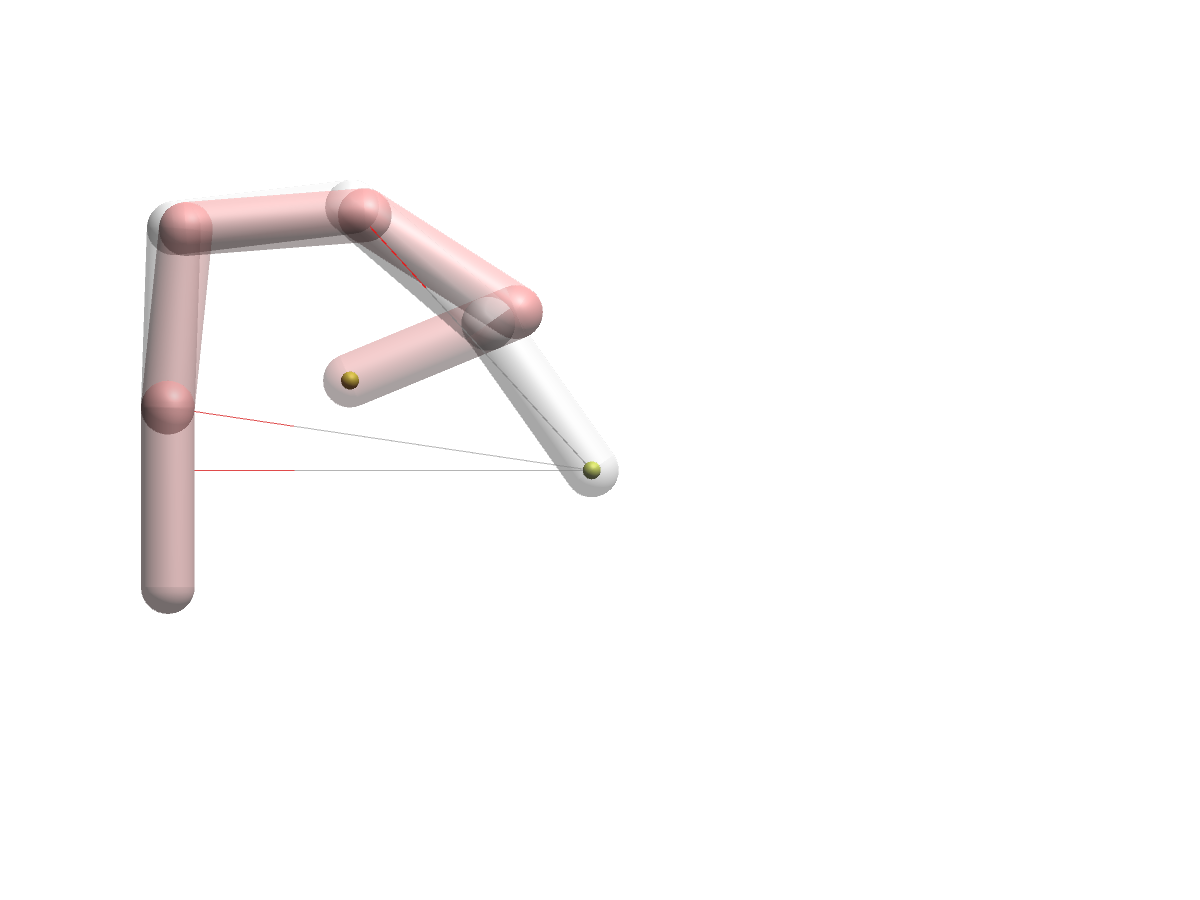
\includegraphics[width=\textwidth]{Figures/distortions/distortions-6.png}
        \caption{$\gamma = -6$}
    \end{subfigure}
    ~
    \begin{subfigure}[b]{.3\textwidth}
        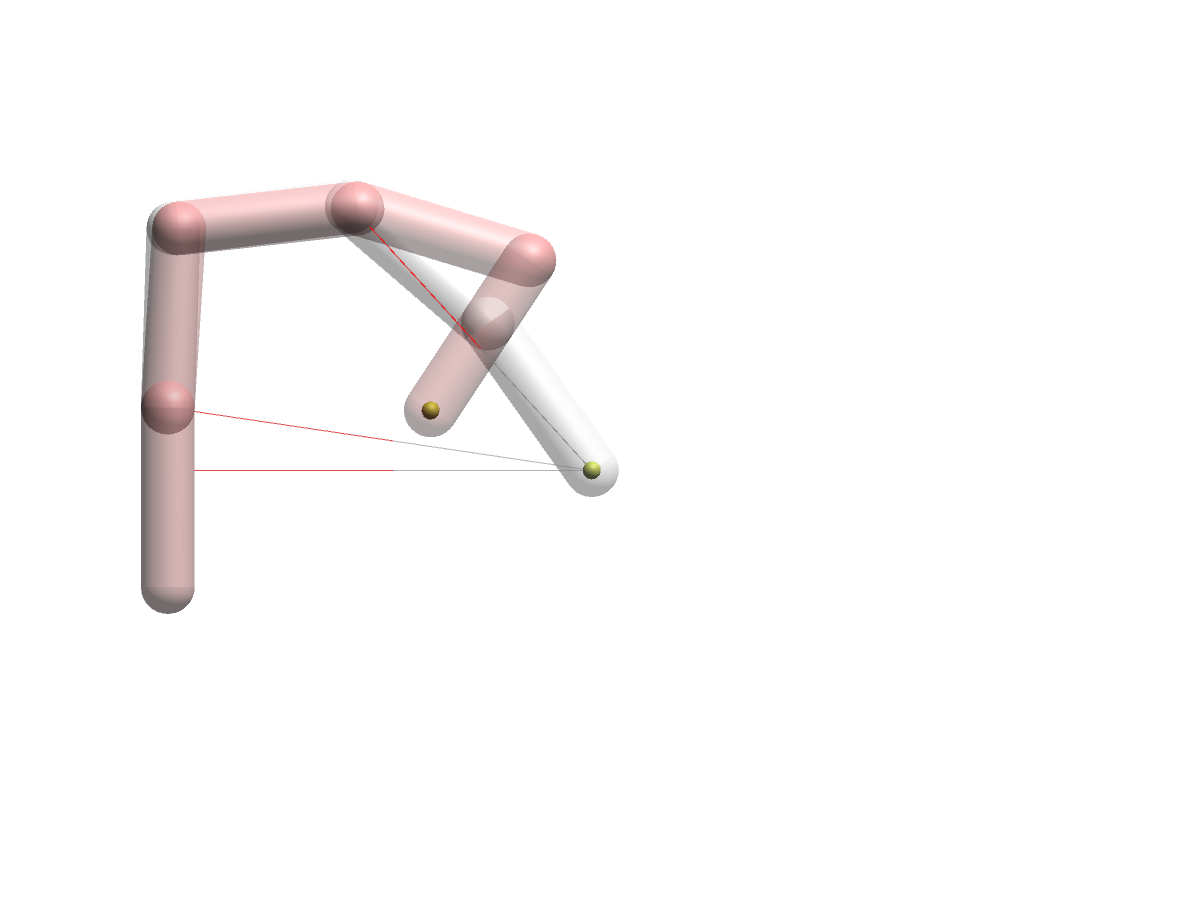
\includegraphics[width=\textwidth]{Figures/distortions/distortions-3.png}
        \caption{$\gamma = -3$}
    \end{subfigure}
    ~
    \begin{subfigure}[b]{.3\textwidth}
        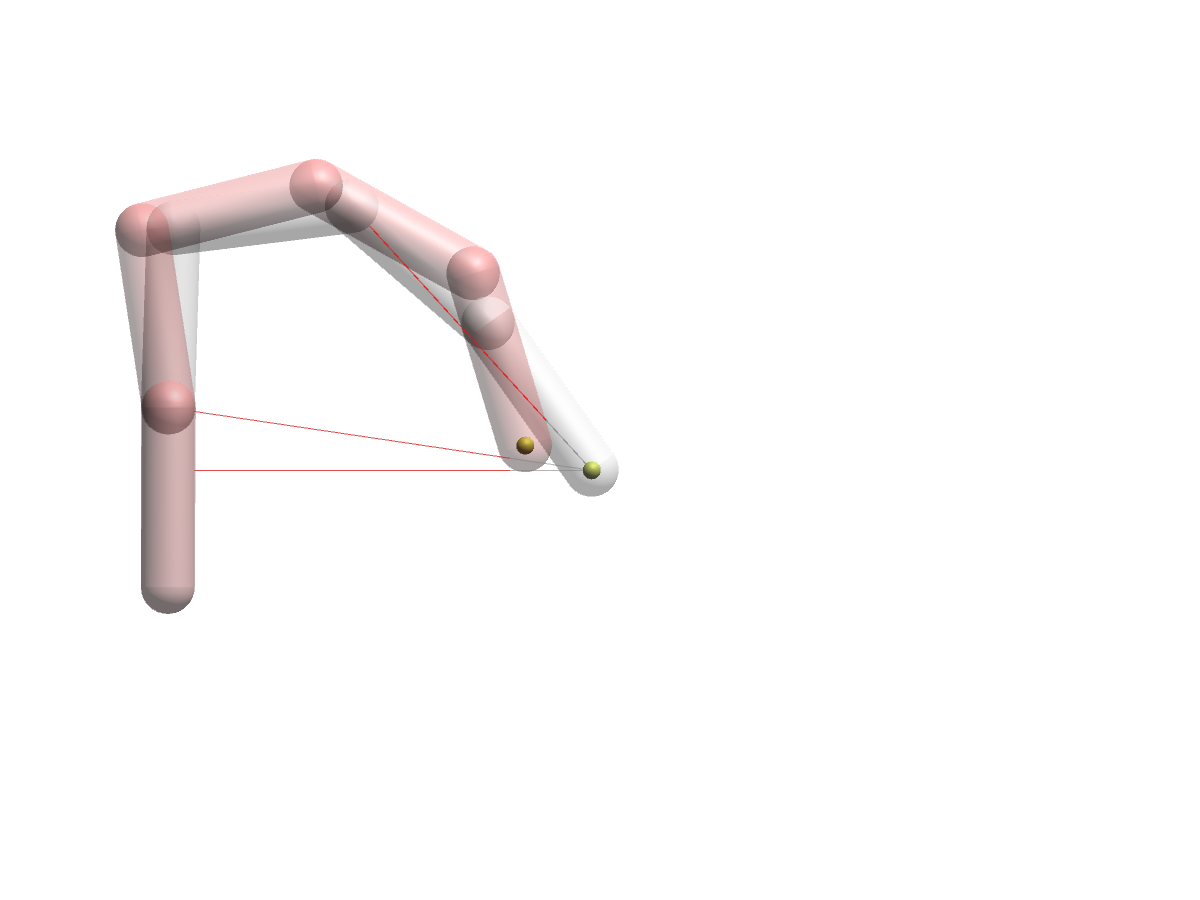
\includegraphics[width=\textwidth]{Figures/distortions/distortions-1.png}
        \caption{$\gamma = -1$}
    \end{subfigure}
    
    
    \begin{subfigure}[b]{.3\textwidth}
        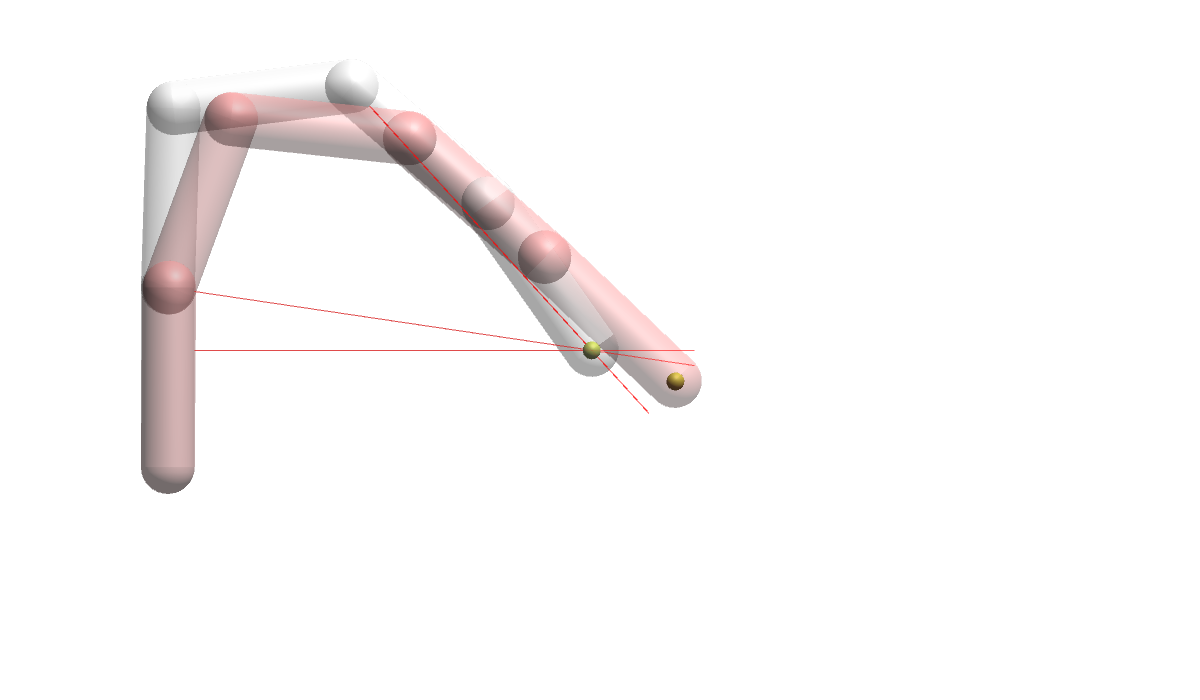
\includegraphics[width=\textwidth]{Figures/distortions/distortions1.png}
        \caption{$\gamma = 1$}
    \end{subfigure}
    ~
    \begin{subfigure}[b]{.3\textwidth}
        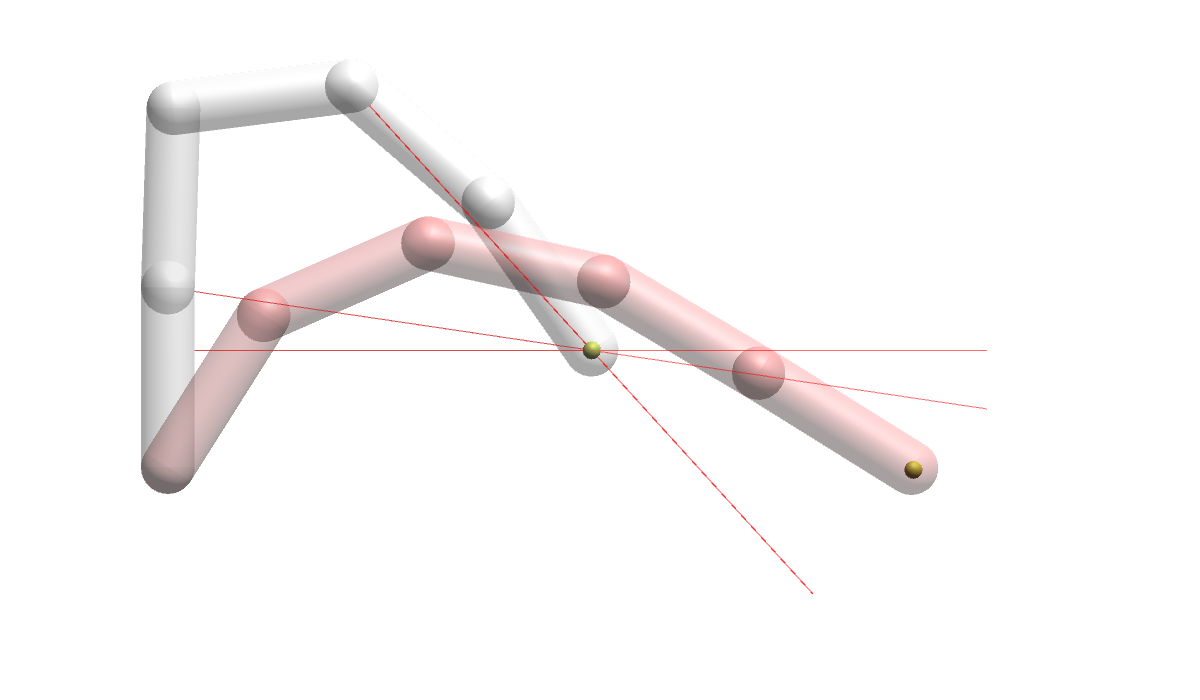
\includegraphics[width=\textwidth]{Figures/distortions/distortions3.png}
        \caption{$\gamma = 3$}
    \end{subfigure}
    ~
    \begin{subfigure}[b]{.3\textwidth}
        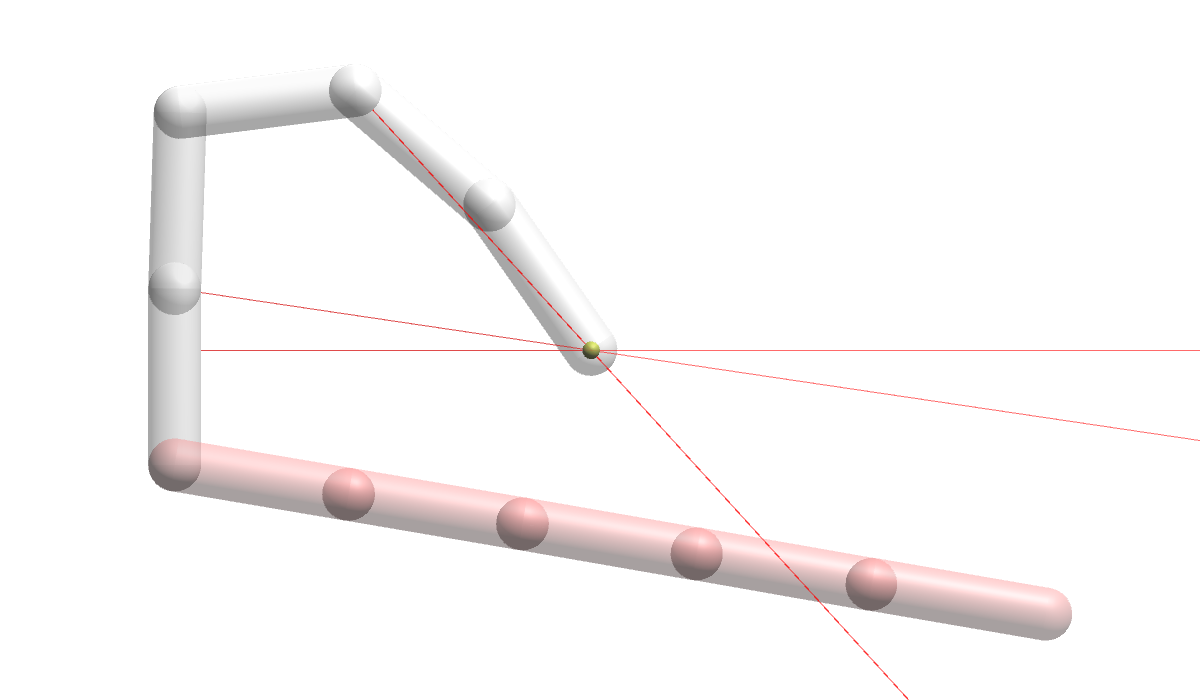
\includegraphics[width=\textwidth]{Figures/distortions/distortions6.png}
        \caption{$\gamma = 6$}
        \label{subfig:gamma6}
    \end{subfigure}
        
    \caption{An example of distorted poses. As always, the captured arms are in gray, the distorted ones in red, and the red and gray lines respectively represent the distorted and original Egocentric coordinates.}
    \label{fig:distortionExamples}
\end{figure}

As one can observe on Figure \ref{fig:distortionExamples}, the distortion works the way it is expected to. As a reminder, a gain of $\pm\SI{6}{\decibel}$ corresponds to a movement whose amplitude is respectively multiplied by $3.981$ and $0.251$, which means it is changed almost fourfold in each direction with respect to a non distorted one. A value of $\gamma = \pm\SI{1}{\decibel}$ similarly modifies a movement by $1.259$ or $0.794$.

The behavior of the arm in Figure \ref{subfig:gamma6} is precisely the one we proposed to avoid using the reachable sphere described in Section \ref{sec:reachableSphere} but we do not report on it here because, as previously justified, we did not implement it in our experiment.

An interactive web application where one may play with both the real arm position and the gain of the distortion, as well as toggling the presence or not of the reachable sphere, is available at \url{https://sidneybovet.github.io/amplified-embodiment/}. The reader is encouraged to play with the IK chain in order to get a better feeling for how the distortion works, especially how it behaves near the skin.

In order to better understand how such a distortion applies to a captured motion, Figure \ref{fig:realMocapDistortion} shows a subject performing a reaching motion towards the air target. The virtual hand is at the same position on all three pictures, but as one may observe, the subject has his hand at different positions. This is due to the fact that in one case (higher hand position) no distortion was applied, while the other (lower hand position) sees a distortion of \SI{3}{\decibel}. The central image shows the superimposition of the two poses in order to better see the position discrepancy.

\begin{figure}[h]
    \centering
    \begin{subfigure}[b]{.3\textwidth}
        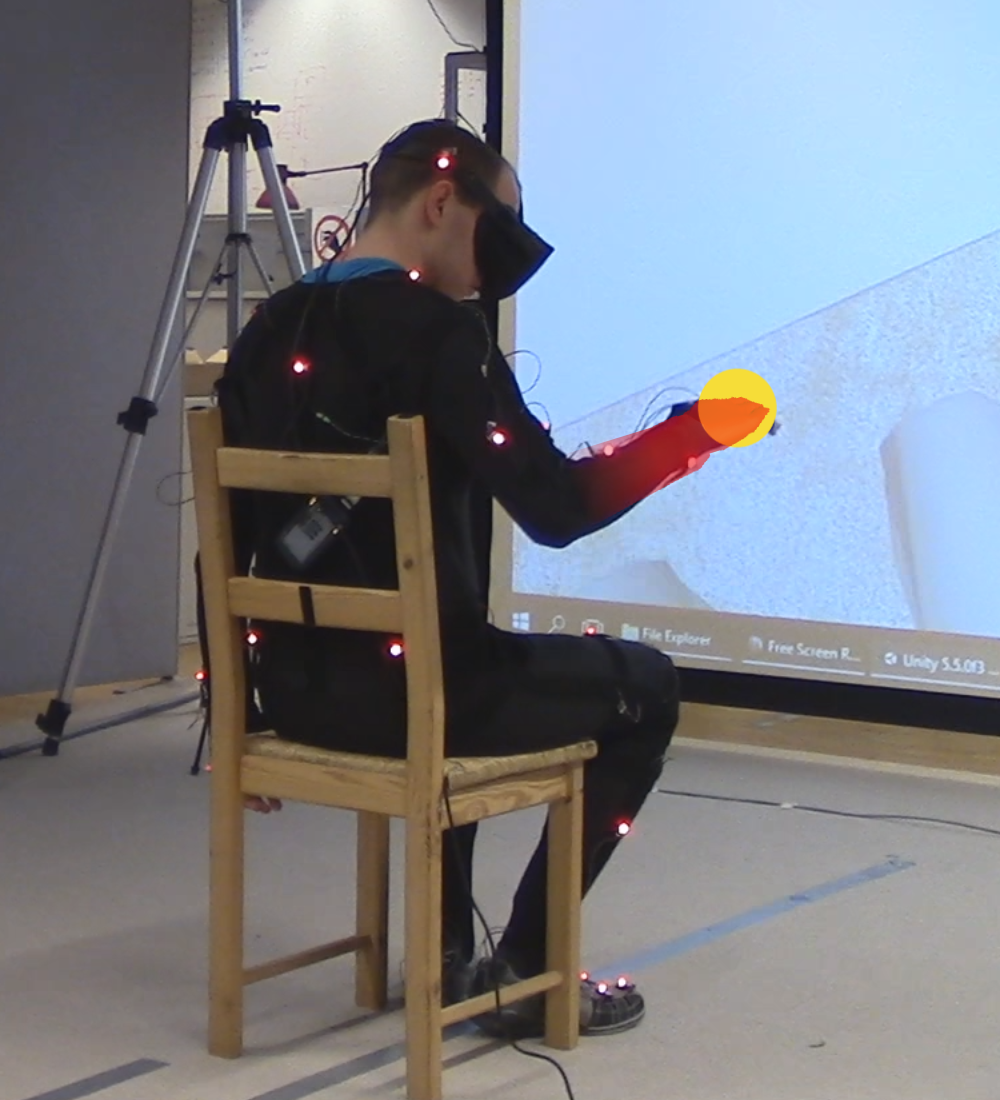
\includegraphics[width=\textwidth]{Figures/handPositionTargetNoDist.png}
    \end{subfigure}
    ~
    \begin{subfigure}[b]{.3\textwidth}
        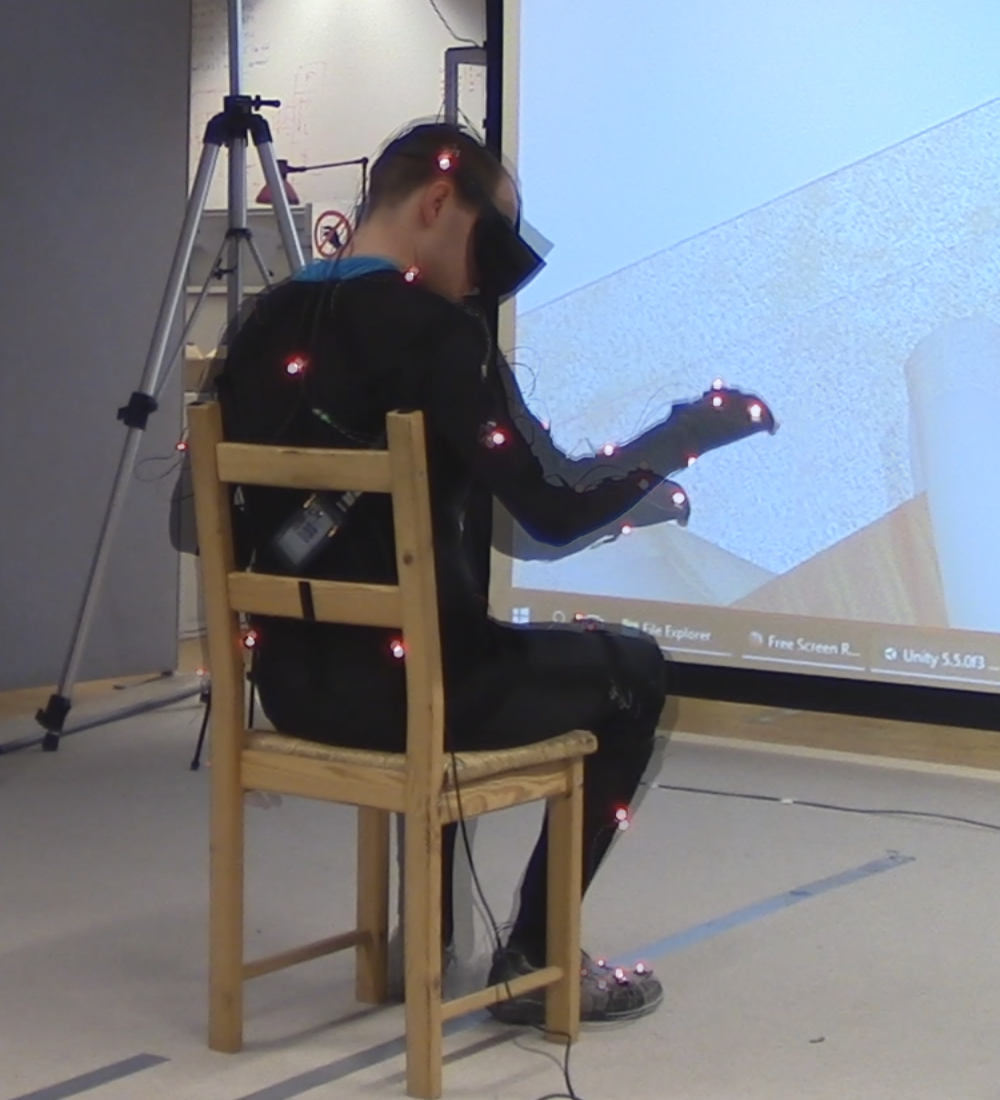
\includegraphics[width=\textwidth]{Figures/handPositionTwice.png}
    \end{subfigure}
    ~
    \begin{subfigure}[b]{.3\textwidth}
        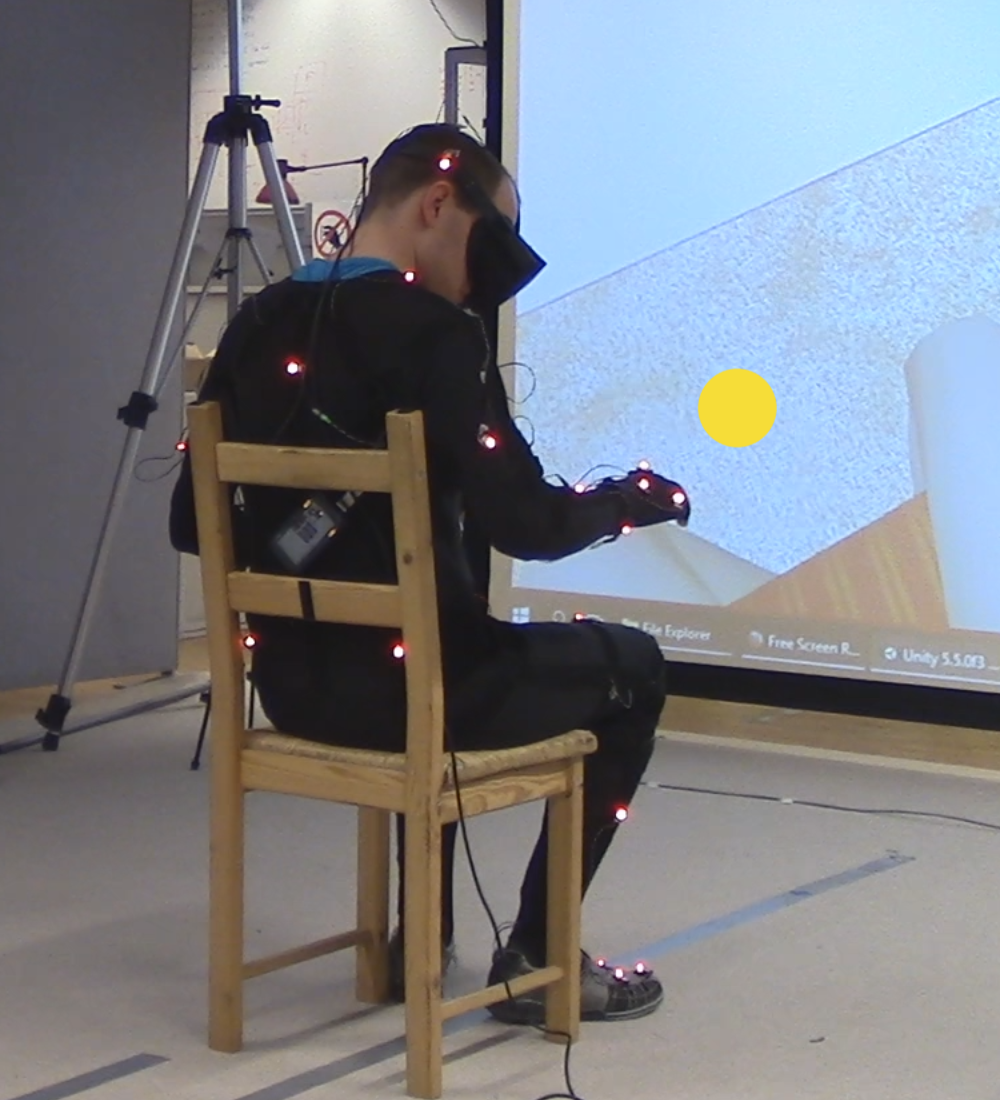
\includegraphics[width=\textwidth]{Figures/handPositionTarget.png}
    \end{subfigure}
        
    \caption{Pictures of a subject, taken from the same point of view, reaching for the same target but with two different distortions of \SI{0}{\decibel} and \SI{3}{\decibel}, with a visual representation of where the target is (yellow dot). The left image shows the \SI{0}{\decibel}, the right one has a distortion of \SI{3}{\decibel}, and the center one is the superimposition of both images.}
    \label{fig:realMocapDistortion}
\end{figure}

This means that in order to perform the same perceived movement, the subject once had to cover the whole distance between his leg and the target, and could in a second time roughly travel two times less in order to reach that target.

\section{Experiment}

---link to the summary video of the experiment---

% Chapter Template

\chapter{Conclusion} % Main chapter title

\label{Chapter6}

\section{Further Work}

--Description of what are the next steps, namely cleaning the toolset, and running the pilot + adjusting the experiment and actually running the experiment--


%----------------------------------------------------------------------------------------
%	THESIS CONTENT - APPENDICES
%----------------------------------------------------------------------------------------

\appendix % Cue to tell LaTeX that the following "chapters" are Appendices

% Include the appendices of the thesis as separate files from the Appendices folder
% Uncomment the lines as you write the Appendices

% Appendix A

\chapter{Questionnaires} % Main appendix title

\label{AppendixA} % For referencing this appendix elsewhere, use \ref{AppendixA}

\section{Characterization Questionnaire}

\begin{table}[h]
  \centering
  \caption{The characterization questionnaire used at the begining of the experiment.}
  \begin{tabular}{| p{.4\textwidth} | m{.6\textwidth} |}
    \hline
    \textbf{Question}                                 & \textbf{Answer} \\ \hline
    Identifier                                        & Numeric answer \\ \hline
    Age                                               & Numeric answer \\ \hline
    Gender                                            & Male / Female \\ \hline
    How often do you participate on experiments
    using Virtual Reality equipments?                 & Never / A few times / Every month / week / day \\ \hline
    How often do you use head mounted displays?       & Never / A few times / Every month / week / day \\ \hline
    How often do you play video games?                & Never / A few times / Every month / week / day \\ \hline
    How often do use the Microsoft Kinect, Nintendo
    Wii or Playstation move?                          & Never / A few times / Every month / week / day \\ \hline
    Hand of preference?                               & Left / Right \\ \hline
    Area(s) of expertise / study / work / interest?   & Text answer \\ \hline
    Are you a student?                                & Bachelor / Master / PhD / No \\ \hline
  \end{tabular}
\end{table}

\section{Detection Question}

The detection question introduced in Chapter \ref{Chapter4} that was asked multiple times to the subjects was the following : ``Did the movements you saw exactly correspond to the movements you performed?''

%% Appendix Template

\chapter{Results} % Main appendix title

\label{AppendixB} % Change X to a consecutive letter; for referencing this appendix elsewhere, use \ref{AppendixX}

Results will be fully shown here.


%----------------------------------------------------------------------------------------
%	BIBLIOGRAPHY
%----------------------------------------------------------------------------------------

\printbibliography[heading=bibintoc]

%----------------------------------------------------------------------------------------

\end{document}
